This problem goal was to simulate Simon's rich-gets-richer model and to see how the simulations match up to the theoretical expectations for the model. In this case I simulated the models for probabilities $p=[0.1, 0.01, 0.001]$ I performed these sumulations with 20,000 samples and repeated the simulation 100 times, combining the output results. From those output results I performed linear regrssion on them to determine the $\alpha$ values to compare them against the expected results. I first had to perform filtering on the tail of the distribution because the range of the distribution is highly dependent on the length of the simulation.

To correlate the results of the simulations and the predictions of the models, the following are used to correlate the values of the slope $\gamma$ to the probability of mutation $\rho$  in terms of the value of $\alpha$.

\[
  \alpha = 
  \frac{1}{\gamma - 1}
  \addtag
\]

\[
  \alpha =
  1 - \rho
  \addtag
\]

\[
  1 - \rho
  =
  \frac{1}{\gamma - 1}
  \addtag
\]

\[
  \gamma - 1
  =
  \frac{1}{1 - \rho}
  \addtag
\]

\[
  \gamma
  =
  \frac{1}{1 - \rho} + 1
  \addtag
\]

Using these equations I can compare the values of the expected and measured values for $\gamma$ for the different mutation rates.

\begin{center}
\begin{tabular}{| c | c | c |}
  \hline
  $\rho$ & $\gamma$ (expected) & $\gamma$ (measured) \\
  \hline
  0.1   & 2.111 & 0.9277 \\
  0.01  & 2.010 & 1.227  \\
  0.001 & 2.001 & 2.559  \\
  \hline
\end{tabular}
\end{center}

My data shows no clear correlaction of any of the expected results from the model. I don't have a good answer for that, but it shows no clear trend for $\gamma \to 2$ as $\rho \to 0$.

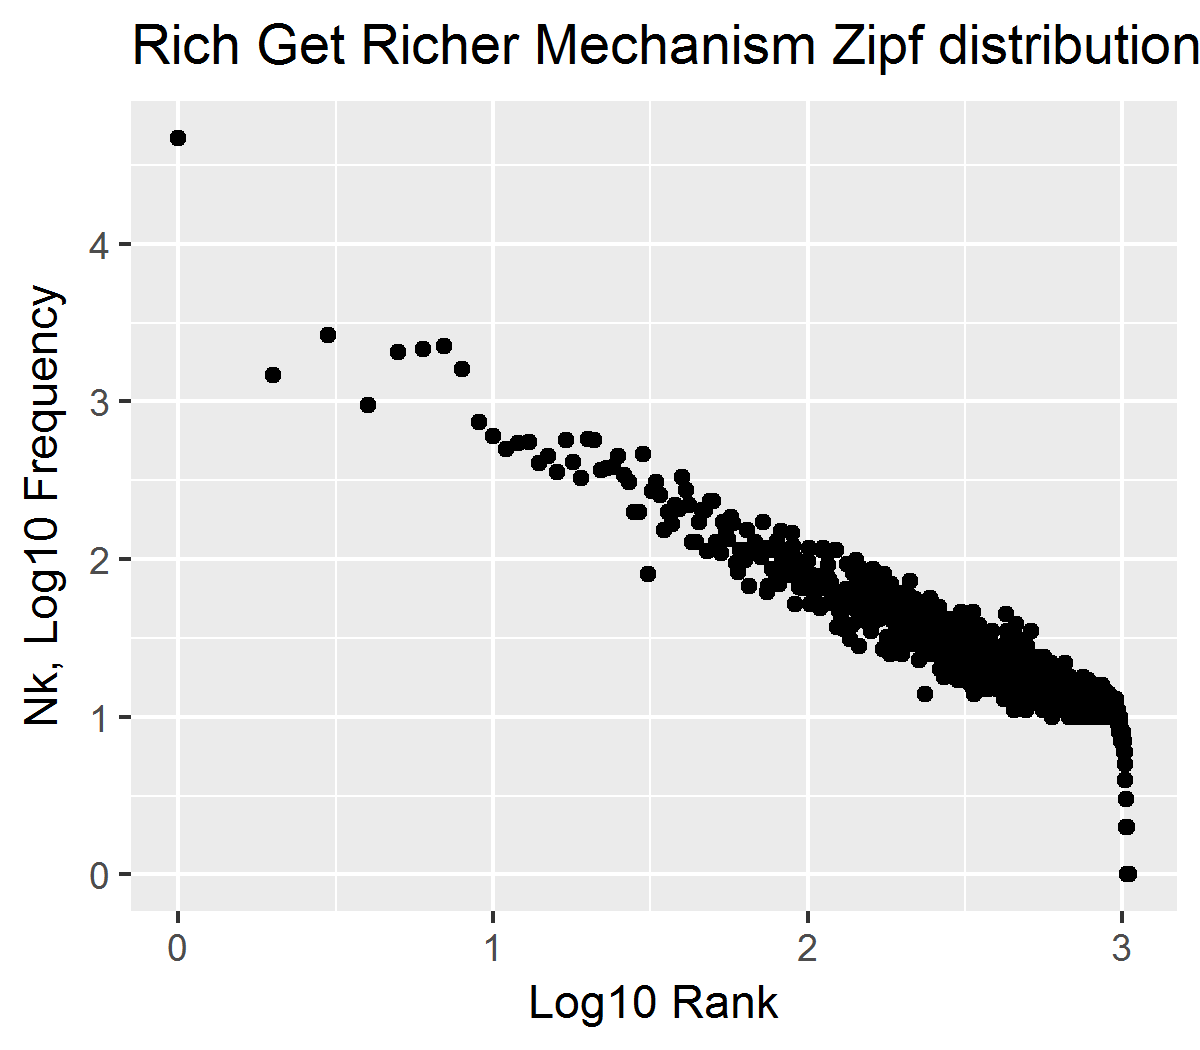
\includegraphics{../images/Problem1_p0_1.png}

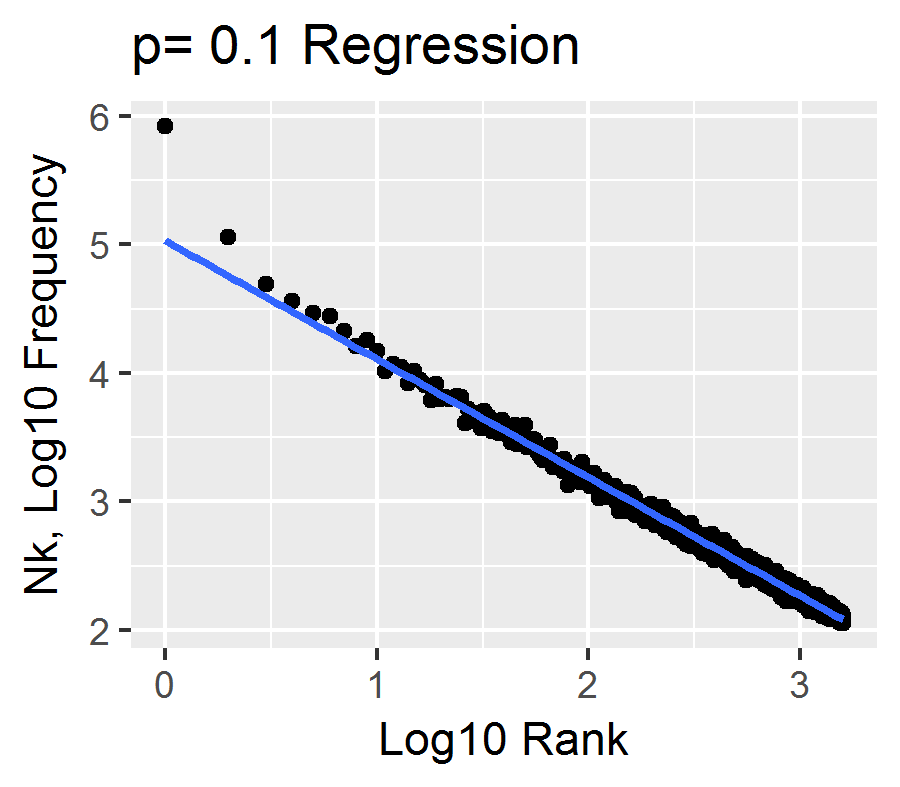
\includegraphics{../images/Problem1_p0_1_lm.png}

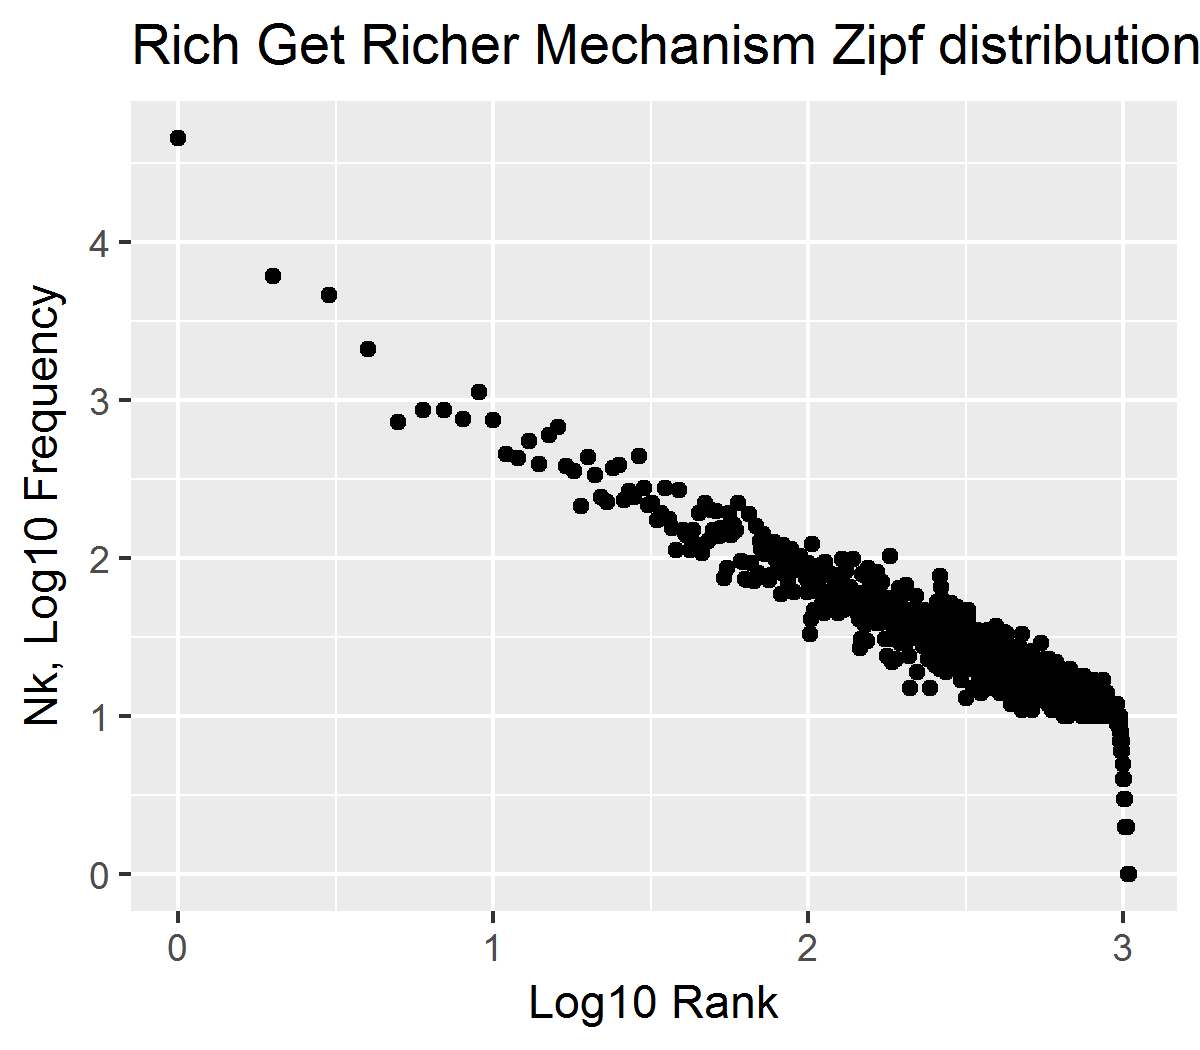
\includegraphics{../images/Problem1_p0_01.png}

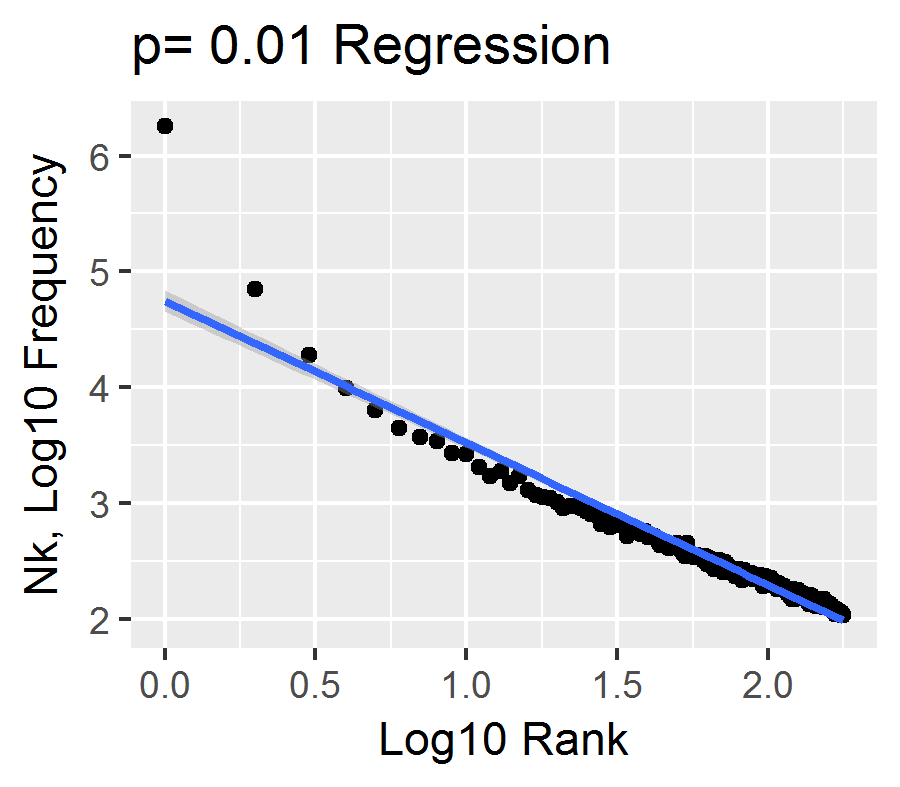
\includegraphics{../images/Problem1_p0_01_lm.png}

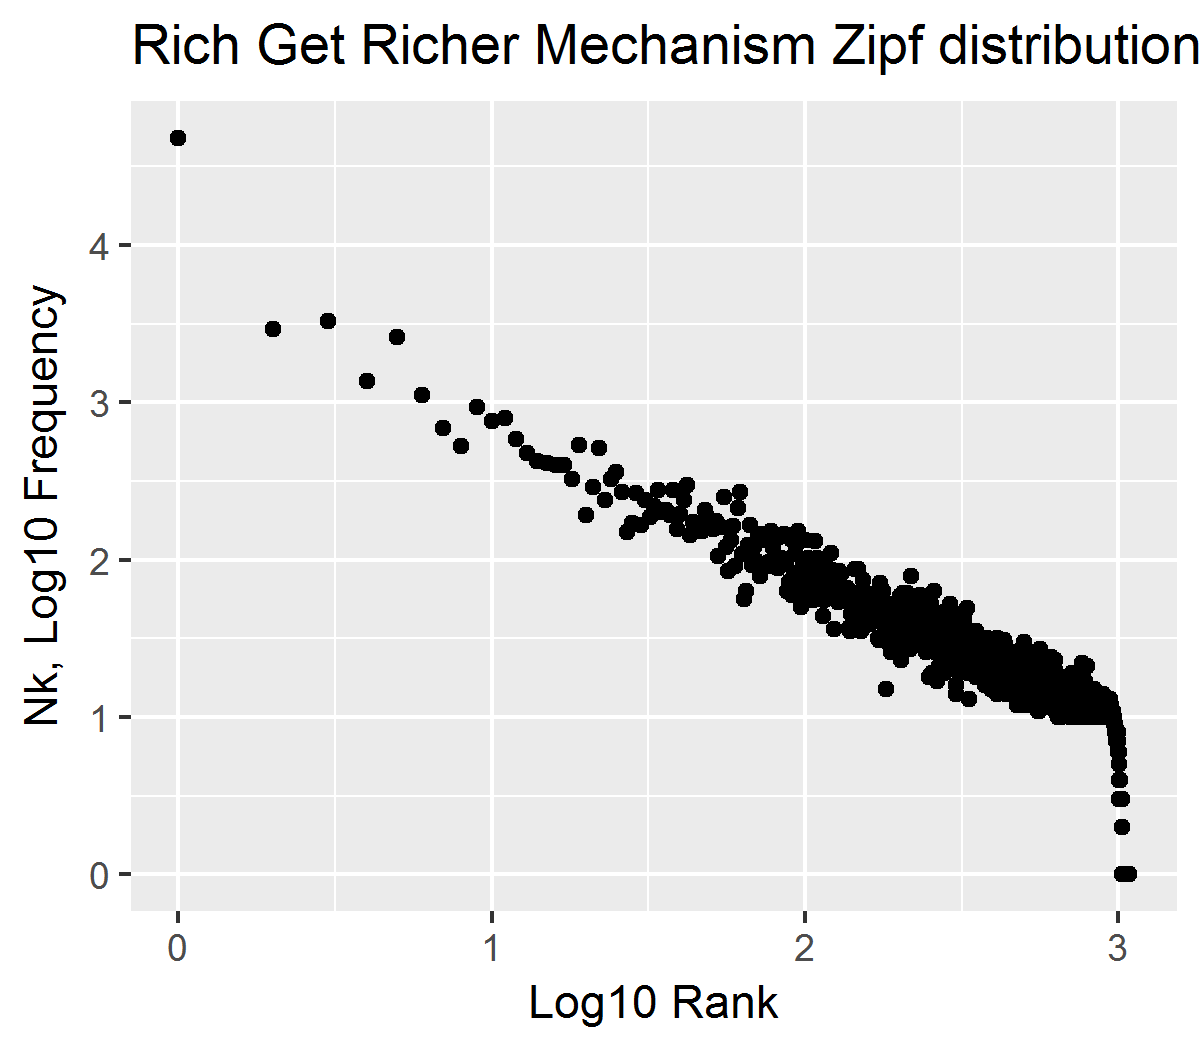
\includegraphics{../images/Problem1_p0_001.png}4

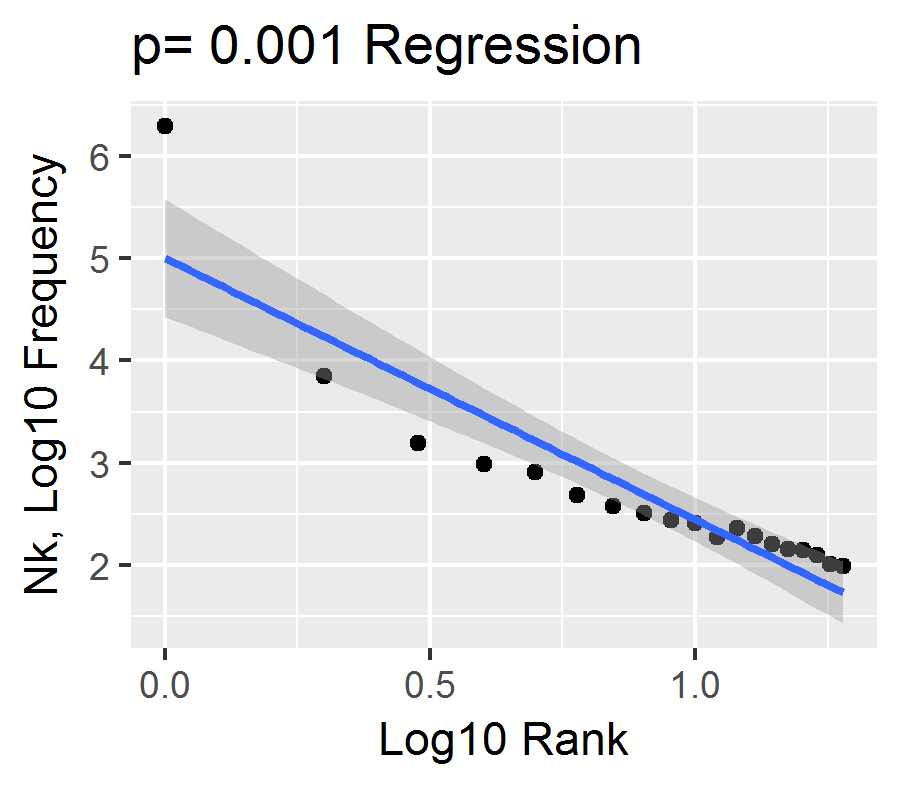
\includegraphics{../images/Problem1_p0_001_lm.png}
